\chapter{Synthèse et optimisation des circuits séquentiels}
\section{Classes et représentation}
Rappelons que l'état du système n'est pas forcement visible par l'extérieur.\\
La sortie d'un système est fonction de l'état et \textit{éventuellement} des entrées. Cet \textit{éventuellement} implique 2 classes de circuit logique séquentiel:
\begin{itemize}
	\item Machine de Moore (pas Gordon!)
	\item Machine de Meally
\end{itemize}
\paragraph{Machine de Moore:}
la \textbf{sortie} est \textbf{uniquement} fonction des \textbf{variables d'état}. Nous n'allons pour le moment que travailler avec des machines de Moore
\begin{figure}[H]
	\centering
	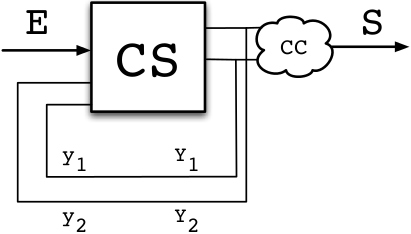
\includegraphics[width=.3\textwidth]{ch7/image1}
\end{figure}
\paragraph{Machine de Meally:}
la \textbf{sortie} est fonction (combinatoire) des \textbf{variables d'état} et des \textbf{entrées}.
\begin{figure}[H]
	\centering
	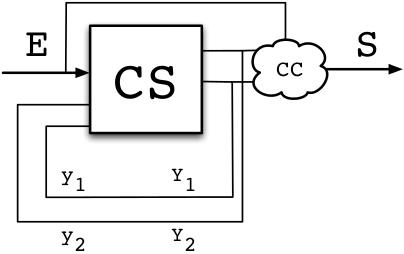
\includegraphics[width=.3\textwidth]{ch7/image2}
\end{figure}

Pour la synthèse à partir d'un cahier de charges verbal :
\begin{enumerate}
	\item Table d'état
	\item Graphe d'état (optionnel)
	\item Équations logiques (et le circuit logique)
\end{enumerate}
\subsection{Codage des états}
On souhaite représenter les systèmes séquentiels à l'aide des codes binaires $\{0, 1, \text{-}\}$. Ce processus d'attribution de codes binaires aux états codés s'appelle \textit{le codage des états}.\\
Le nombre de bits nécessaires pour coder $n$ états est donné par $\log_2n$.
\subsubsection{Exemple}
Soit un système à 4 états. Attribuons à chaque état un code binaire (4 états $\rightarrow \log_2 4=2\rightarrow$ 2 bits nécessaires).\\
Ainsi $1\rightarrow 00\ ;\ 2\rightarrow 01\ ;\ 3\rightarrow 11\ ;\ 4\rightarrow 10$.\\
Ainsi, on obtient:
\begin{figure}[H]
	\centering
	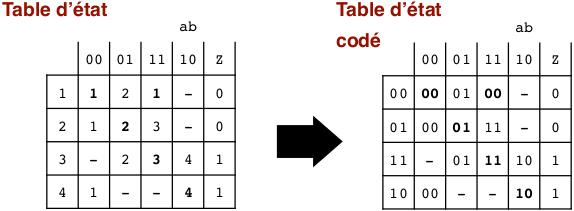
\includegraphics[width=.6\textwidth]{ch7/image3}
\end{figure}
À chaque bit du code correspond une fonction logique. On a donc : 4 états, 2 variables d'états ($y_2y_1$)$\rightarrow$ 2 fonctions logiques.
\begin{figure}[H]
	\centering
	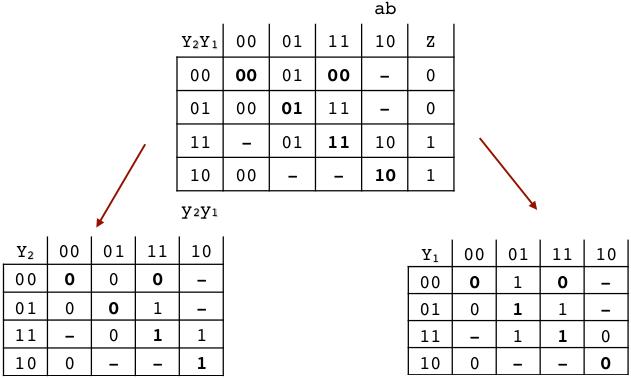
\includegraphics[width=.7\textwidth]{ch7/image4}
\end{figure}
Il suffit de simplifier la K-Map de $Y_2$ et celle de $Y_1$ et déduire leur fonction logique respective
\begin{figure}[H]
	\centering
	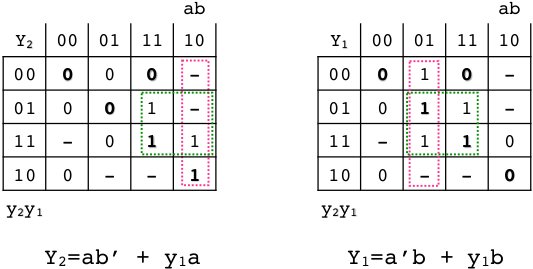
\includegraphics[width=.7\textwidth]{ch7/image5}
\end{figure}
\danger $y_2y_1\neq Y_2Y_1$, les premières représentent le présent, les 2 autres le futur.\\

Établissons la \textit{fonction de sortie}. Connaissant la valeur de sortie des états stables, nous pouvons remplir les cases correspondantes.
\begin{figure}[H]
	\centering
	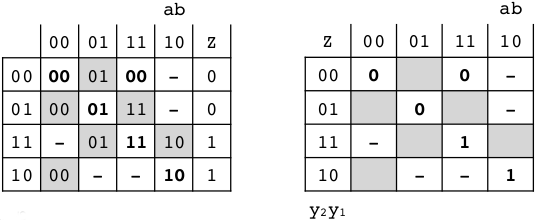
\includegraphics[width=.7\textwidth]{ch7/image6}
\end{figure} Pour les transitions (cases grises), il faut respecter les transitions ainsi que la règle suivante:
\begin{center}
	\textbf{Lors des transitions, si la sortie doit changer, elle ne devrait changer qu'une seule fois}
\end{center}
c-à-d que les \textbf{seules} possibilités sont
\begin{figure}[H]
	\centering
	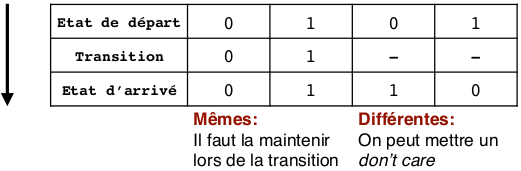
\includegraphics[width=.7\textwidth]{ch7/image7}
\end{figure}
Nous obtenons donc
\begin{figure}[H]
	\centering
	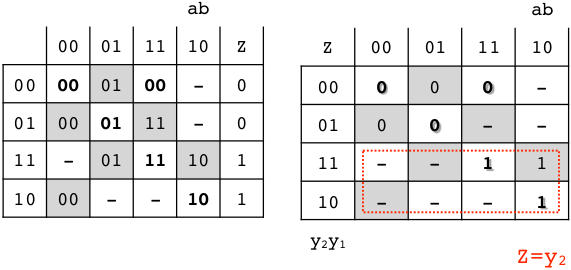
\includegraphics[width=.7\textwidth]{ch7/image8}
\end{figure}
Le logigramme correspondant n'est autre que
\begin{figure}[H]
	\centering
	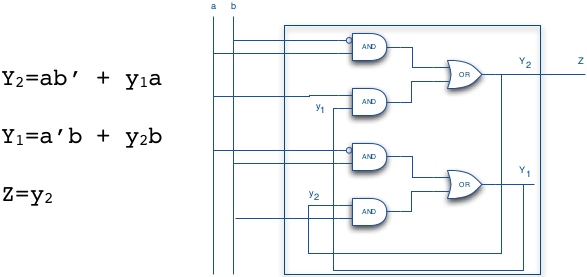
\includegraphics[width=.8\textwidth]{ch7/image9}
\end{figure}
\section{Simplification de la table primitive des états}

\section{Synthèse d'un flip-flop D}

\section{Différents organes de mémoire}